\documentclass[xcolor={table}]{beamer}
\usepackage{fleqn}
\usepackage{graphicx}
\usepackage{coordsys} %for \numbline commander

%Setup appearance:
\usetheme{Darmstadt}
\usefonttheme[onlylarge]{structurebold}
\setbeamerfont*{frametitle}{size=\normalsize,series=\bfseries}
\setbeamertemplate{navigation symbols}{}
\setbeamertemplate{bibliography item}{[\theenumiv]}

% Standard packages
\usepackage[english]{babel}
\usepackage[latin1]{inputenc}
\usepackage{times}
\usepackage[T1]{fontenc}
\usepackage{multirow}
\usepackage{subfigure}
\usepackage{pbox}
\usepackage{arydshln}
\usepackage{pifont}
\usepackage{cancel}
\usepackage{rotating} % for sideways headings

% Source Code packages
\usepackage{algorithm2e}
\usepackage{algorithmic}

\DeclareSymbolFont{extraup}{U}{zavm}{m}{n}
\DeclareMathSymbol{\varclub}{\mathalpha}{extraup}{84}
\DeclareMathSymbol{\varspade}{\mathalpha}{extraup}{85}
\DeclareMathSymbol{\varheart}{\mathalpha}{extraup}{86}
\DeclareMathSymbol{\vardiamond}{\mathalpha}{extraup}{87}

%%% This section command that adds a big page with section dividers
\usepackage{xifthen}% provides \isempty test
\newcommand{\SectionSlide}[2][]{
	\ifthenelse{\isempty{#1}}
		{\section{#2}\begin{frame} \begin{center}\begin{huge}#2\end{huge}\end{center}\end{frame}}
		{\section[#1]{#2}\begin{frame} \begin{center}\begin{huge}#2\end{huge}\end{center}\end{frame}}
}
%Extends the section slide to to include a shortened section title for the navigation bar as a second parameter
\newcommand{\SectionSlideShortHeader}[3][]{
	\ifthenelse{\isempty{#1}}
		{\section[#3]{#2}\begin{frame} \begin{center}\begin{huge}#2\end{huge}\end{center}\end{frame}}
		{\section[#1]{#2}\begin{frame} \begin{center}\begin{huge}#3\end{huge}\end{center}\end{frame}}
}

\newcommand{\refer}[1]{\footnote{#1}}
\newcommand{\GW}{\text{\textit{Guess-Who~}}}
\newcommand{\keyword}[1]{\alert{\textbf{#1}}\index{#1}}
\newcommand{\firstkeyword}[1]{\textbf{#1}\index{#1}}
\newcommand{\indexkeyword}[1]{\alert{\textbf{#1}\index{#1}}}
\newcommand{\featN}[1]{\textsc{#1}}
\newcommand{\featL}[1]{\textit{'#1'}}
 \newcommand{\ourRef}[1]{\ref{#1} $^{\text{\tiny[\pageref{#1}]}}$}
 \newcommand{\ourEqRef}[1]{\eqref{#1}$^{\text{\tiny[\pageref{#1}]}}$}
  
\DeclareMathOperator*{\argmax}{argmax}
\DeclareMathOperator*{\argmin}{argmin}

\title{Data to Insights to Decisions}
	\author{John D. Kelleher and Brian Mac Namee and Aoife D'Arcy}
\institute{}
	\date{}
\begin{document}
\begin{frame}
	\titlepage
\end{frame}
\begin{frame}
	 \tableofcontents
\end{frame}

\SectionSlideShortHeader{Converting Business Problems into Analytics Solutions}{Problems to Solutions}

\begin{frame}
\begin{itemize}
\item Converting a business problem into an analytics solution involves answering the following key questions:
\begin{enumerate}
\item What is the business problem?
\item What are the goals that the business wants to achieve?
\item How does the business currently work?
\item In what ways could a predictive analytics model help to address the business problem?
\end{enumerate}
\end{itemize}
\end{frame}

\subsection{Case Study: Motor Insurance Fraud}


\begin{frame}
\begin{block}{Case Study: Motor Insurance Fraud}
In spite of having a fraud investigation team that investigates up to $30$\% of all claims made, a  motor insurance company is still losing too much money due to fraudulent claims. 
\end{block}
\begin{itemize}
	\item What predictive analytics solutions could be proposed to help address this business problem?
\end{itemize}
\end{frame}

\begin{frame}
\begin{itemize}
	\item Potential analytics solutions include:
\begin{itemize}
	\item Claim prediction 
	\item Member prediction
	\item Application prediction
	\item Payment prediction 
\end{itemize}
\end{itemize}
\end{frame}

\SectionSlide{Assessing Feasibility}

\begin{frame}
\begin{itemize}
\item Evaluating the feasibility of a proposed analytics solution involves considering the following questions:
\begin{enumerate}
\item Is the data required by the solution available, or could it be made available? 
\item What is the capacity of the business to utilize the insights that the analytics solution will provide?
\end{enumerate}
\end{itemize}
\end{frame}

\subsection{Case Study: Motor Insurance Fraud}

\begin{frame}[plain]
\begin{itemize}
	\item What are the data and capacity requirements for the proposed Claim Prediction analytics solution for the motor insurance fraud scenario?
\end{itemize}
\pause
\begin{block}{Case Study: Motor Insurance Fraud}
\textbf{[Claim prediction]}\\
\textit{Data Requirements:} A large collection of historical claims marked as \featL{fraudulent} and \featL{non-fraudulent}. Also, the details of each claim, the related policy, and the related claimant would need to be available. 
~\\
\textit{Capacity Requirements:} The main requirement is that a mechanism could be put in place to inform claims investigators that some claims were prioritized above others. This would also require that information about claims become available in a suitably timely manner so that the claims investigation process would not be delayed by the model.
\end{block}
\end{frame}

\SectionSlideShortHeader{Designing the Analytics Base Table}{ABT Design}
 
\begin{frame} 
\begin{itemize}
\item The basic structure in which we capture historical datasets is the \keyword{analytics base table} (\keyword{ABT})
\end{itemize}
\begin{figure}[htb]
       \begin{centering}
       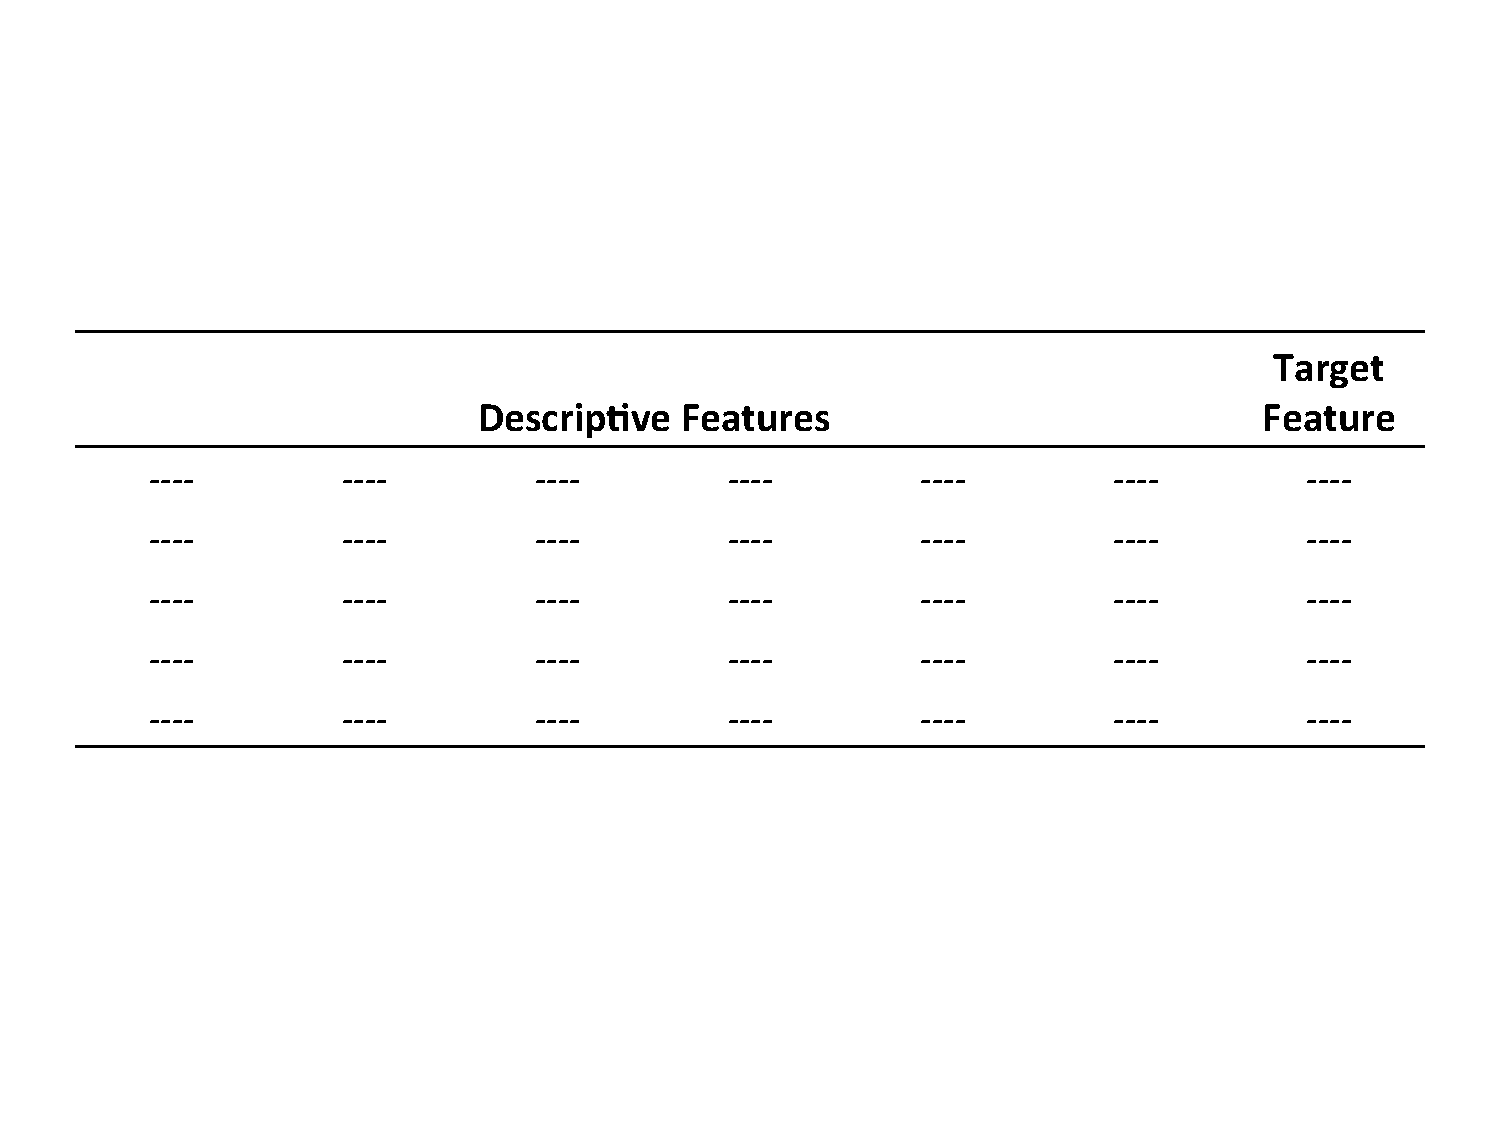
\includegraphics[width=0.8\textwidth]{images/AnalyticsBaseTable2.pdf}
       \caption{The general structure of an \keyword{analytics base table}---descriptive features and a target feature.}
       \label{fig:analyticsBaseTable}
       \end{centering}
\end{figure}
\end{frame} 

 \begin{frame} 
\begin{figure}[htb]
	\begin{center}
			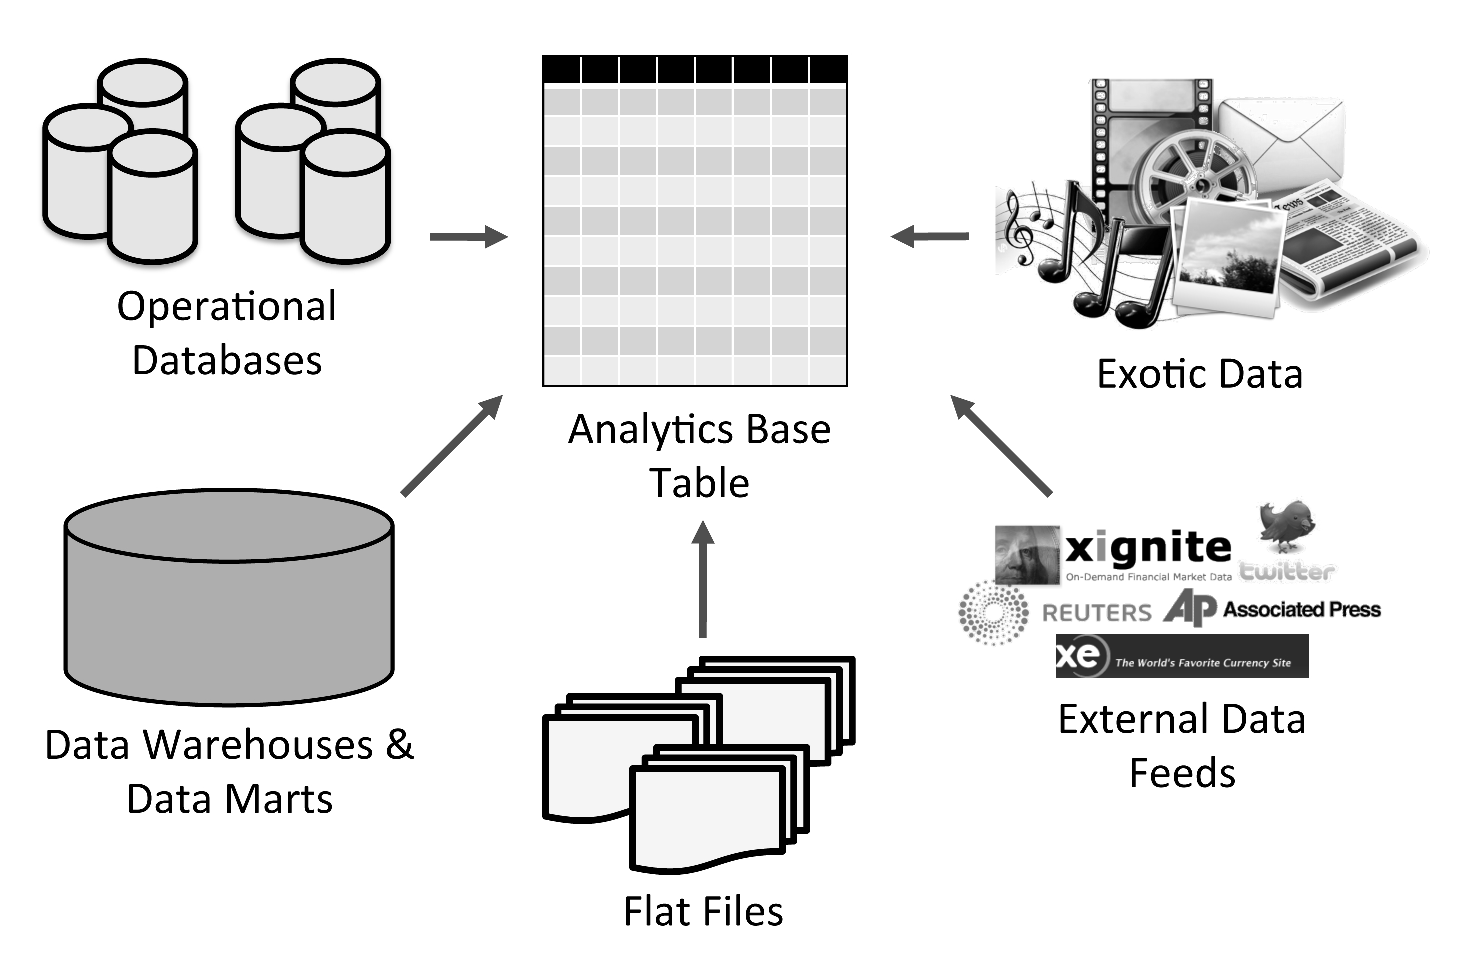
\includegraphics[width=0.8\textwidth]{./images/WhereDoesDataComeFromBW.pdf}
	\end{center}
	\caption{The different data sources typically combined to create an analytics base table.}
	\label{fig:WhereDoesDataComeFrom}
\end{figure}
\end{frame} 

\begin{frame}
\begin{itemize}
\item The \keyword{prediction subject} defines the basic level at which predictions are made, and each row in the ABT will represent one instance of the prediction subject---the phrase \keyword{one-row-per-subject} is often used to describe this structure. 
\item Each row in an ABT is composed of a set of descriptive features and a target feature. 
\item Defining features can be difficult!
\end{itemize}
\end{frame}

\begin{frame}
\begin{itemize}
\item A good way to define features is to identify the key \keyword{domain concepts} and then to base the features on these concepts.
\end{itemize}
\end{frame} 


 \begin{frame} 
\begin{figure}[htb]
	\begin{center}
			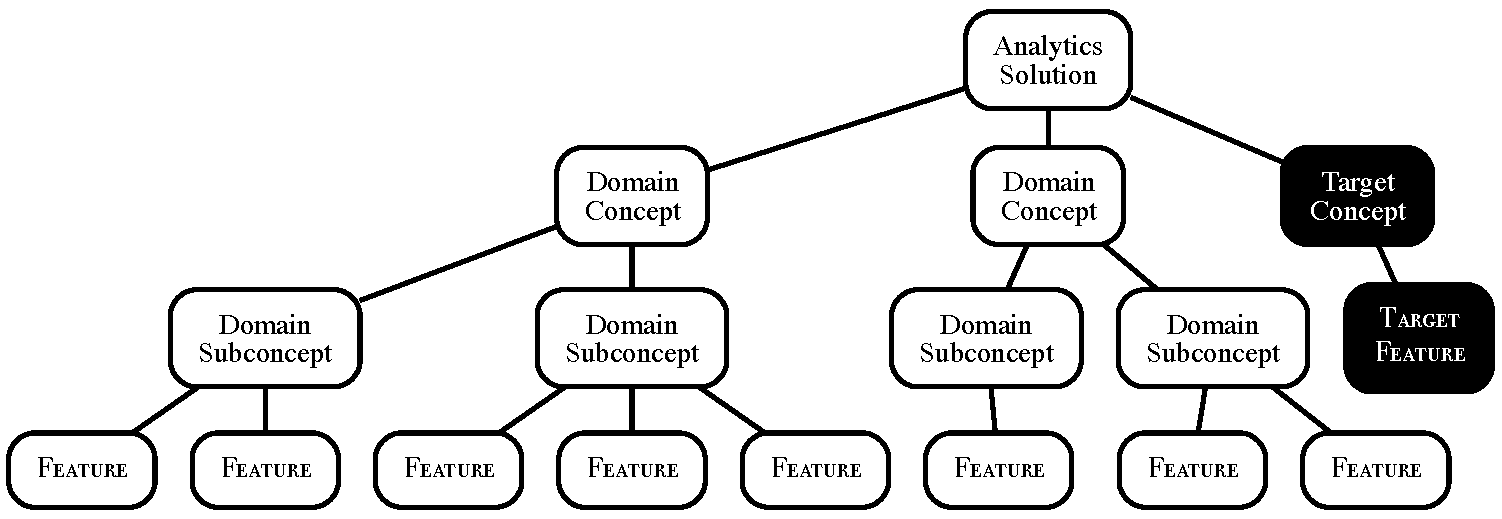
\includegraphics[width=\textwidth]{./images/standardHierarchy_SMCAPS.pdf}
	\end{center}
	\caption{The hierarchical relationship between an analytics solution, domain concepts, and descriptive features.}
	\label{fig:DataMetrics2}
\end{figure}
\end{frame} 

\begin{frame}
\begin{itemize}
\item There are a number of general domain concepts that are often useful:
\begin{itemize}
	\item Prediction Subject Details
	\item Demographics
	\item Usage
	\item Changes in Usage
	\item Special Usage
	\item Lifecycle Phase
	\item Network Links
\end{itemize}
\end{itemize}
\end{frame} 

\subsection{Case Study: Motor Insurance Fraud}

 \begin{frame} 
\begin{figure}[htb]
	\begin{center}
			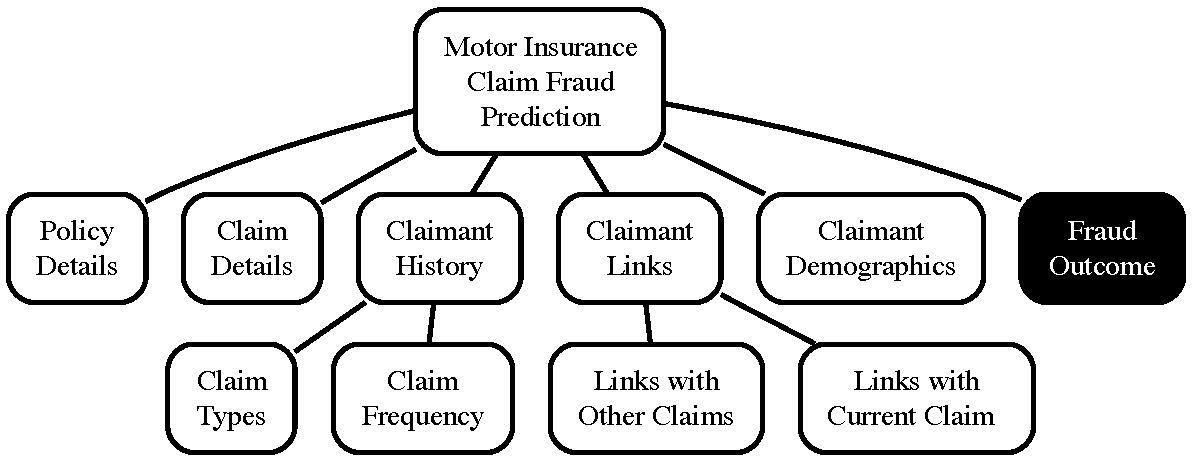
\includegraphics[width=0.9\textwidth]{./images/motorInsurance1.pdf}
	\end{center}
	\caption{Example domain concepts for a motor insurance fraud claim prediction analytics solution.}
	\label{fig:DataMetrics3}
\end{figure}
\end{frame} 

\SectionSlide{Designing \& Implementing Features}


\begin{frame}
\begin{itemize}
\item Three key data considerations are particularly important when we are designing features.
\begin{itemize}
\item \keyword{Data availability}
\item \keyword{Timing}
\item \keyword{Longevity}
\end{itemize}
\end{itemize}
\end{frame} 

\subsection{Different Types of Data}

\begin{frame}
\begin{figure}[htb]
	\centering
			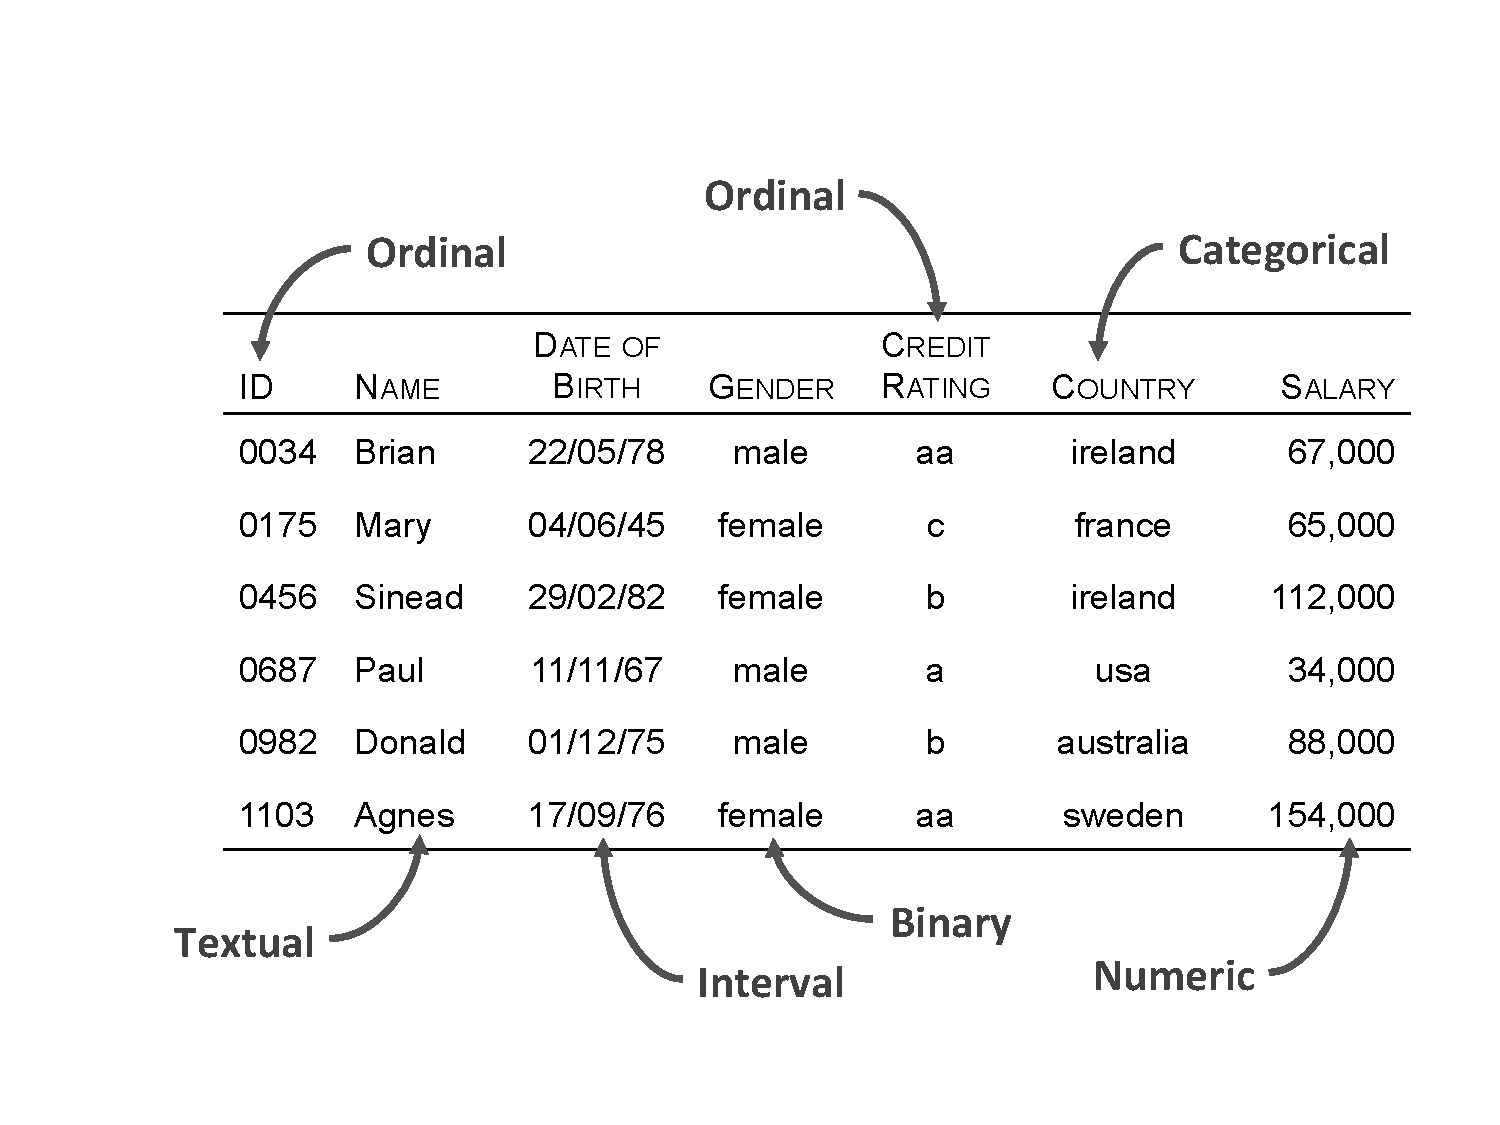
\includegraphics[width=0.8\textwidth]{./images/DataTypes6.pdf}
	\caption{Sample descriptive feature data illustrating numeric, binary, ordinal, interval, categorical, and textual types.}
	\label{fig:dataTypes}
\end{figure}
\end{frame} 


\subsection{Different Types of Features}

\begin{frame}
\begin{itemize}
\item The features in an ABT can be of two types: 
\begin{itemize}
\item \keyword{raw features} 
\item \keyword{derived features} 
\end{itemize}
\item There are a number of common derived feature types:
\begin{itemize}
	\item \keyword{Aggregates}
	\item \keyword{Flags}
	\item \keyword{Ratios}
	\item \keyword{Mappings}
\end{itemize}
\end{itemize}
\end{frame} 

\subsection{Handling Time}


\begin{frame}
\begin{itemize}
\item Many of the predictive models that we build are \keyword{propensity models}, which inherently have a temporal element
\item For \keyword{propensity modeling}, there are two key periods: 
\begin{itemize}
\item the \keyword{observation period}
\item the \keyword{outcome period}
\end{itemize}
\end{itemize}
\end{frame} 

 \begin{frame} [plain]
\begin{itemize}
\item In some cases the observation and outcome period are measured over the same time for all predictive subjects. 
\end{itemize}
\begin{figure}[htb]
	\begin{center}
			\subfigure[Observation period and outcome period]{\label{fig:pointInTimeDiscussion1}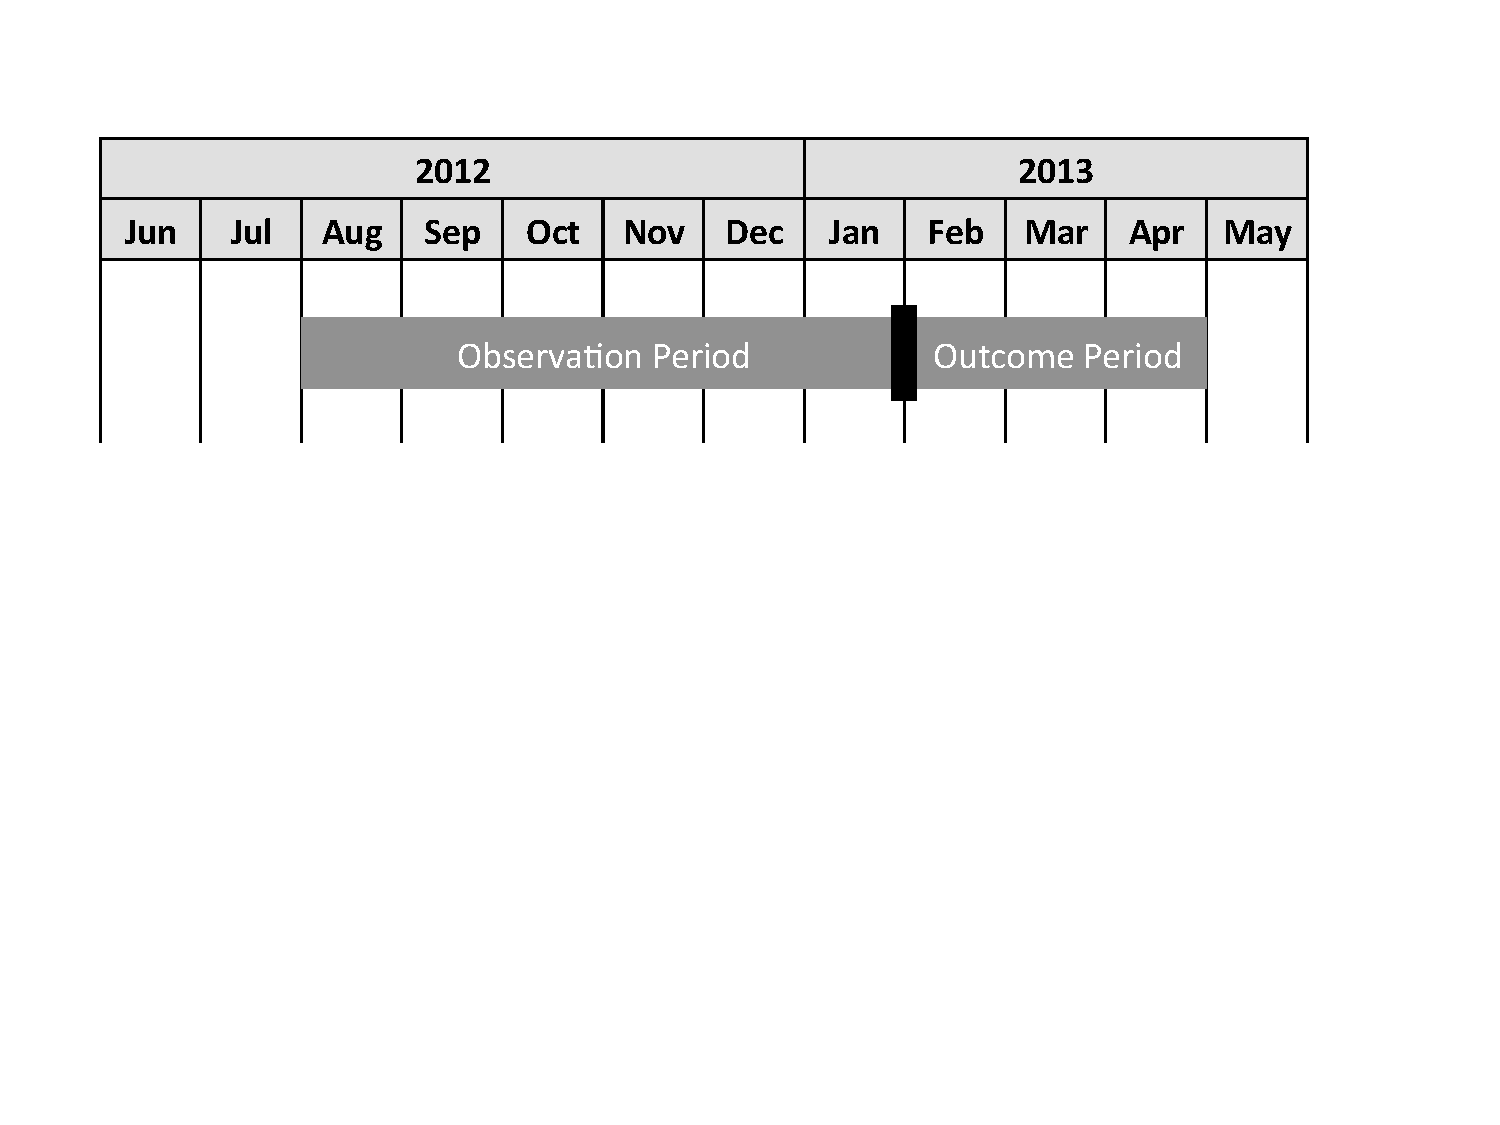
\includegraphics[width=0.5\textwidth]{./images/ModellingTimeBehaviourTargetPeriod2.pdf}}
			\subfigure[Observation and outcome periods for multiple customers (each line represents a customer)]{\label{fig:pointInTimeDiscussion2}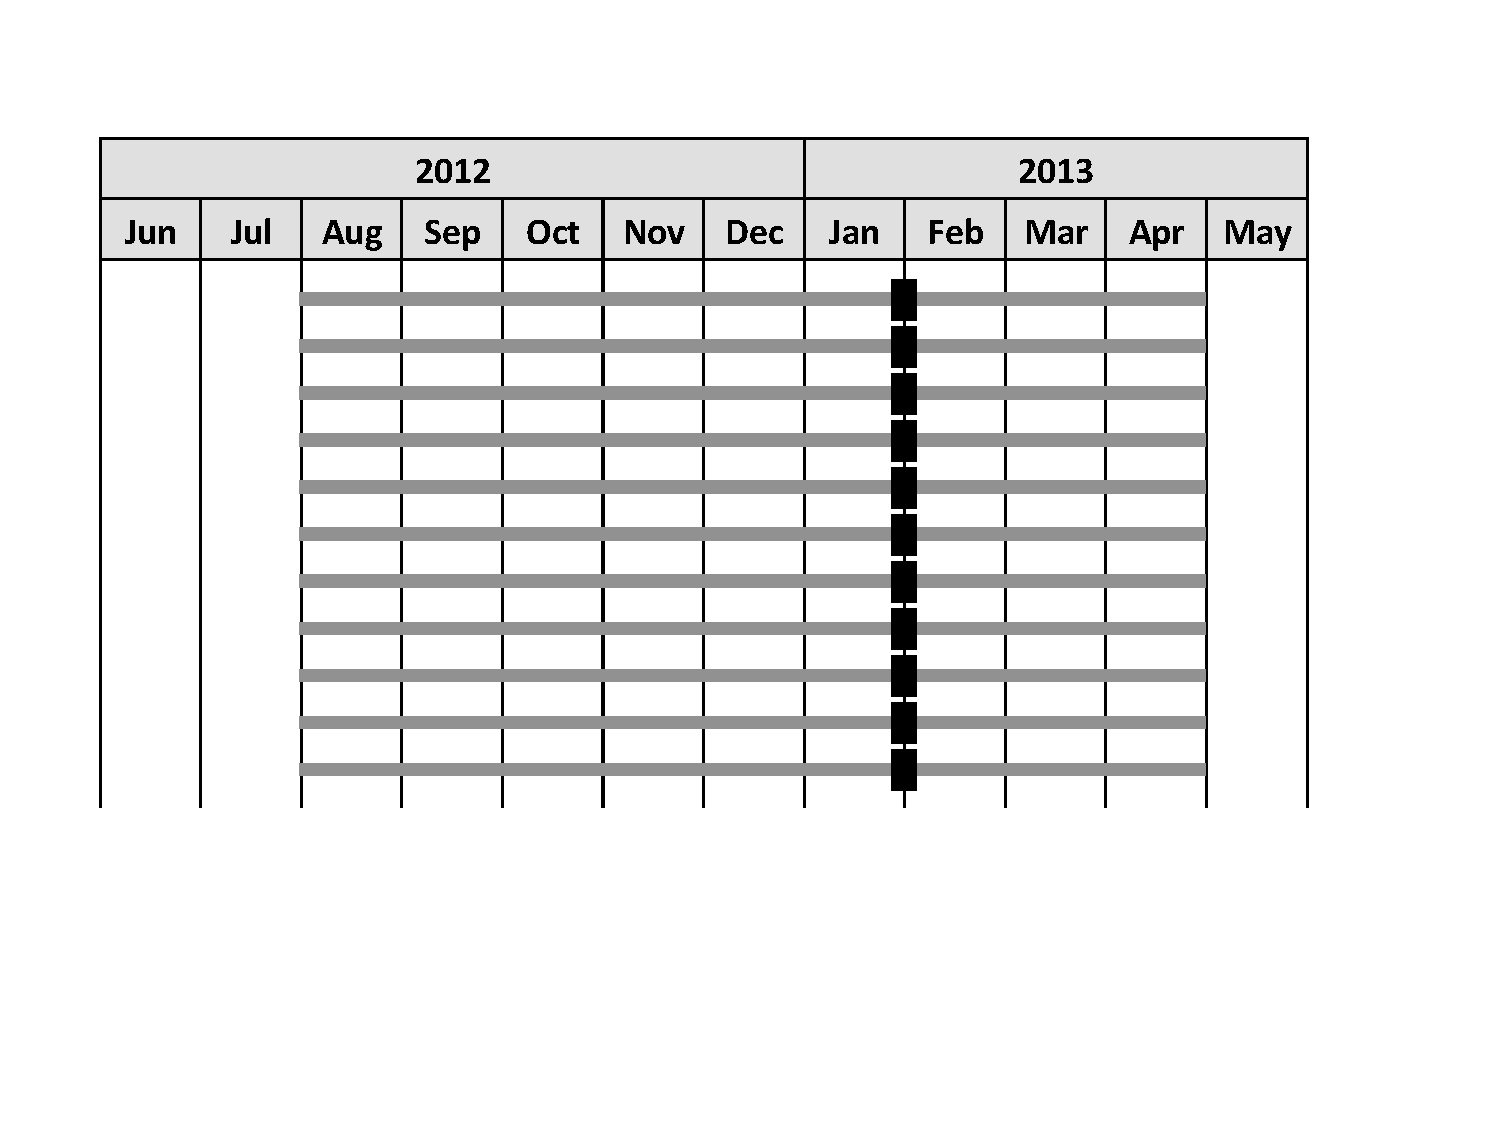
\includegraphics[width=0.5\textwidth]{./images/ModellingTimeBehaviourThenOutcome.pdf}}
	\end{center}
	\caption{Modeling points in time.}
	\label{fig:pointInTimeDiscussion}
\end{figure}
\end{frame} 


\begin{frame}
\begin{itemize}
\item Often the observation period and outcome period will be measured over different dates  for each prediction subject. 
\end{itemize}
\begin{figure}[htb]
	\begin{center}
			\subfigure[Actual]{\label{fig:pointInTimeEventThenOutcome1}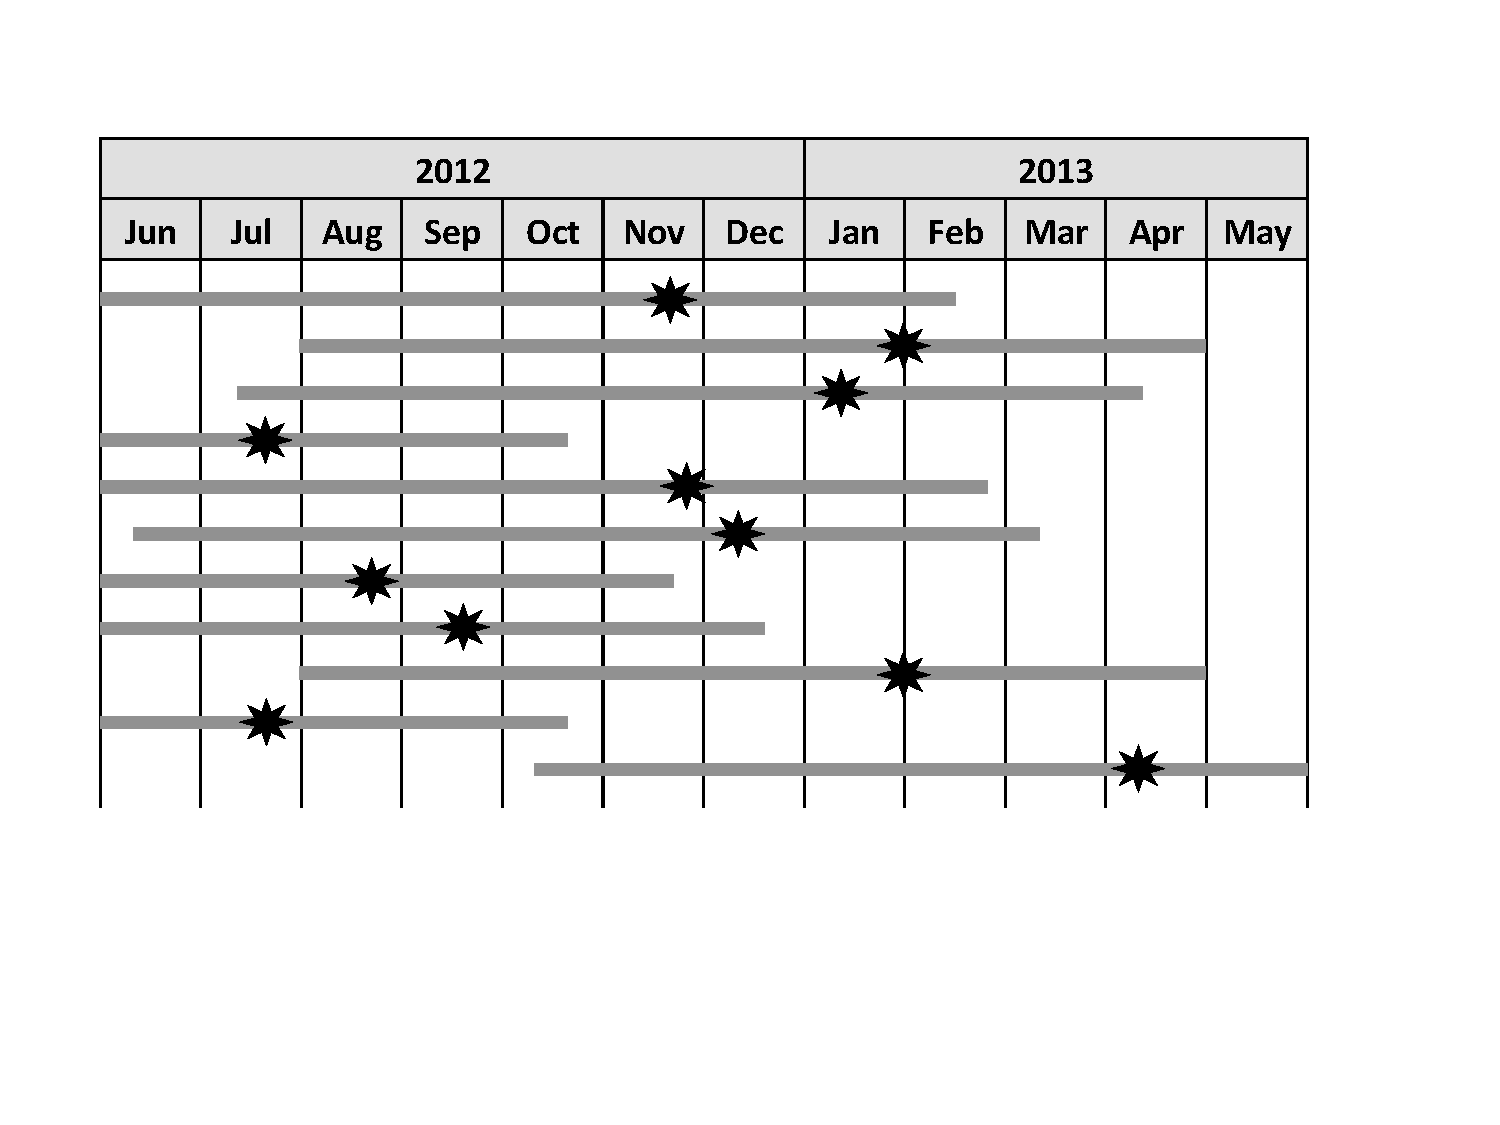
\includegraphics[width=0.49\textwidth]{./images/ModellingTimeBehaviourThenEventThenOutcome.pdf}}
			\subfigure[Aligned]{\label{fig:pointInTimeEventThenOutcome2}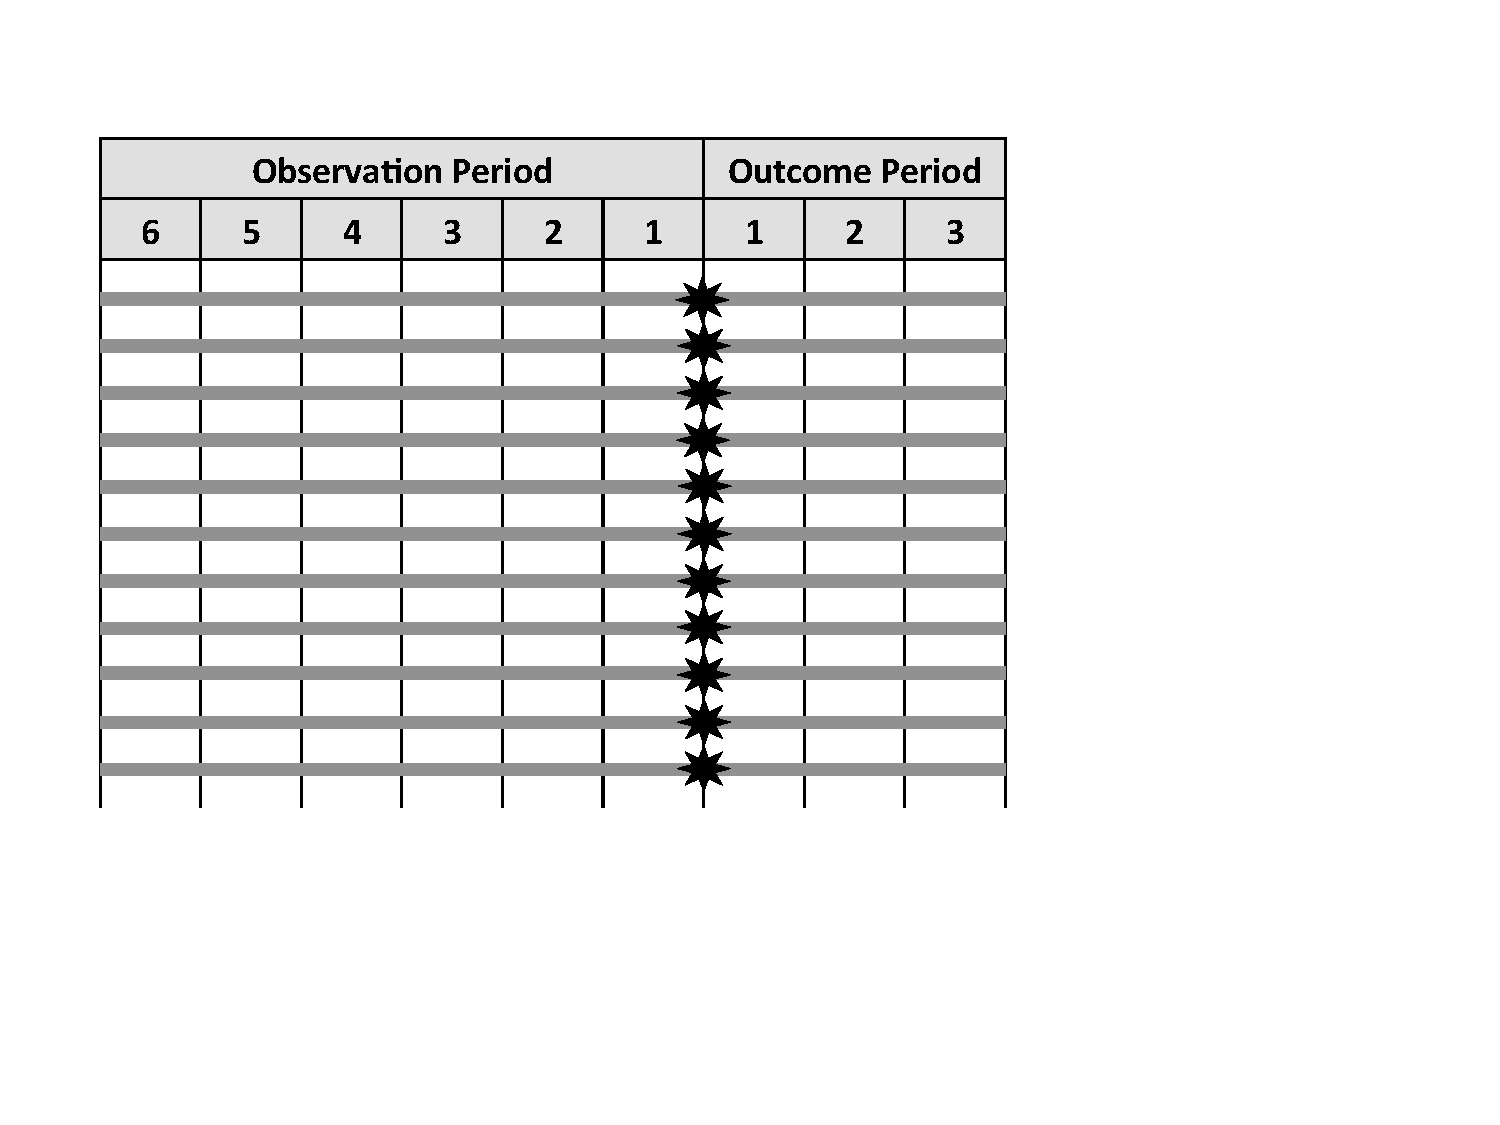
\includegraphics[width=0.37\textwidth]{./images/ModellingTimeBehaviourThenEventThenOutcomeAligned.pdf}}
	\end{center}
	\caption{Observation and outcome periods defined by an event rather than by a fixed point in time  (each line represents a prediction subject and stars signify events).}
	\label{fig:pointInTimeEventThenOutcome}
\end{figure}
\end{frame} 

%

\begin{frame}
\begin{itemize}
\item In some cases only the descriptive features have a time component to them, and the target feature is time independent.
\end{itemize}
\begin{figure}[htb]
	\begin{center}
			%\subfigure[]{\label{fig:pointInTimeDiscussion3}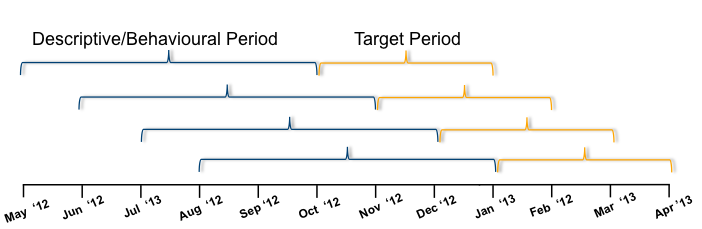
\includegraphics[width=0.32\textwidth]{./images/DataPointInTimeDiscussion05.png}}
			\subfigure[Actual]{\label{fig:pointInTimeDiscussion4}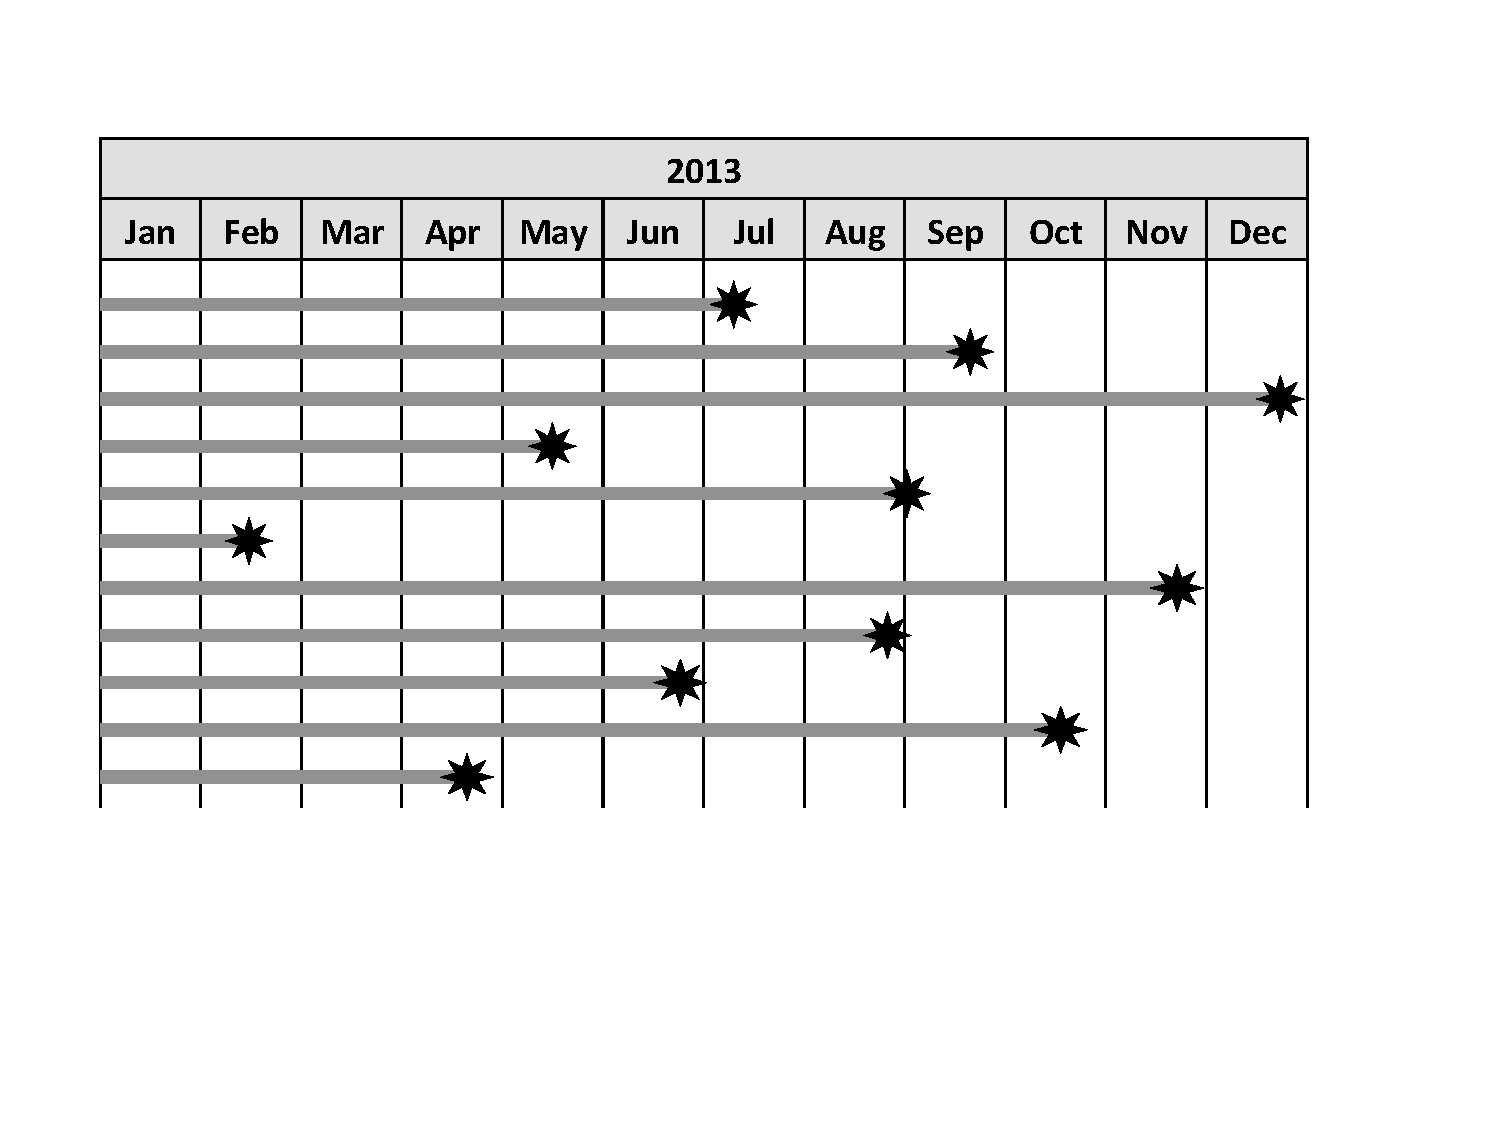
\includegraphics[width=0.49\textwidth]{./images/ModellingTimeBehaviourThenEvent2.pdf}}
			\subfigure[Aligned]{\label{fig:pointInTimeDiscussion5}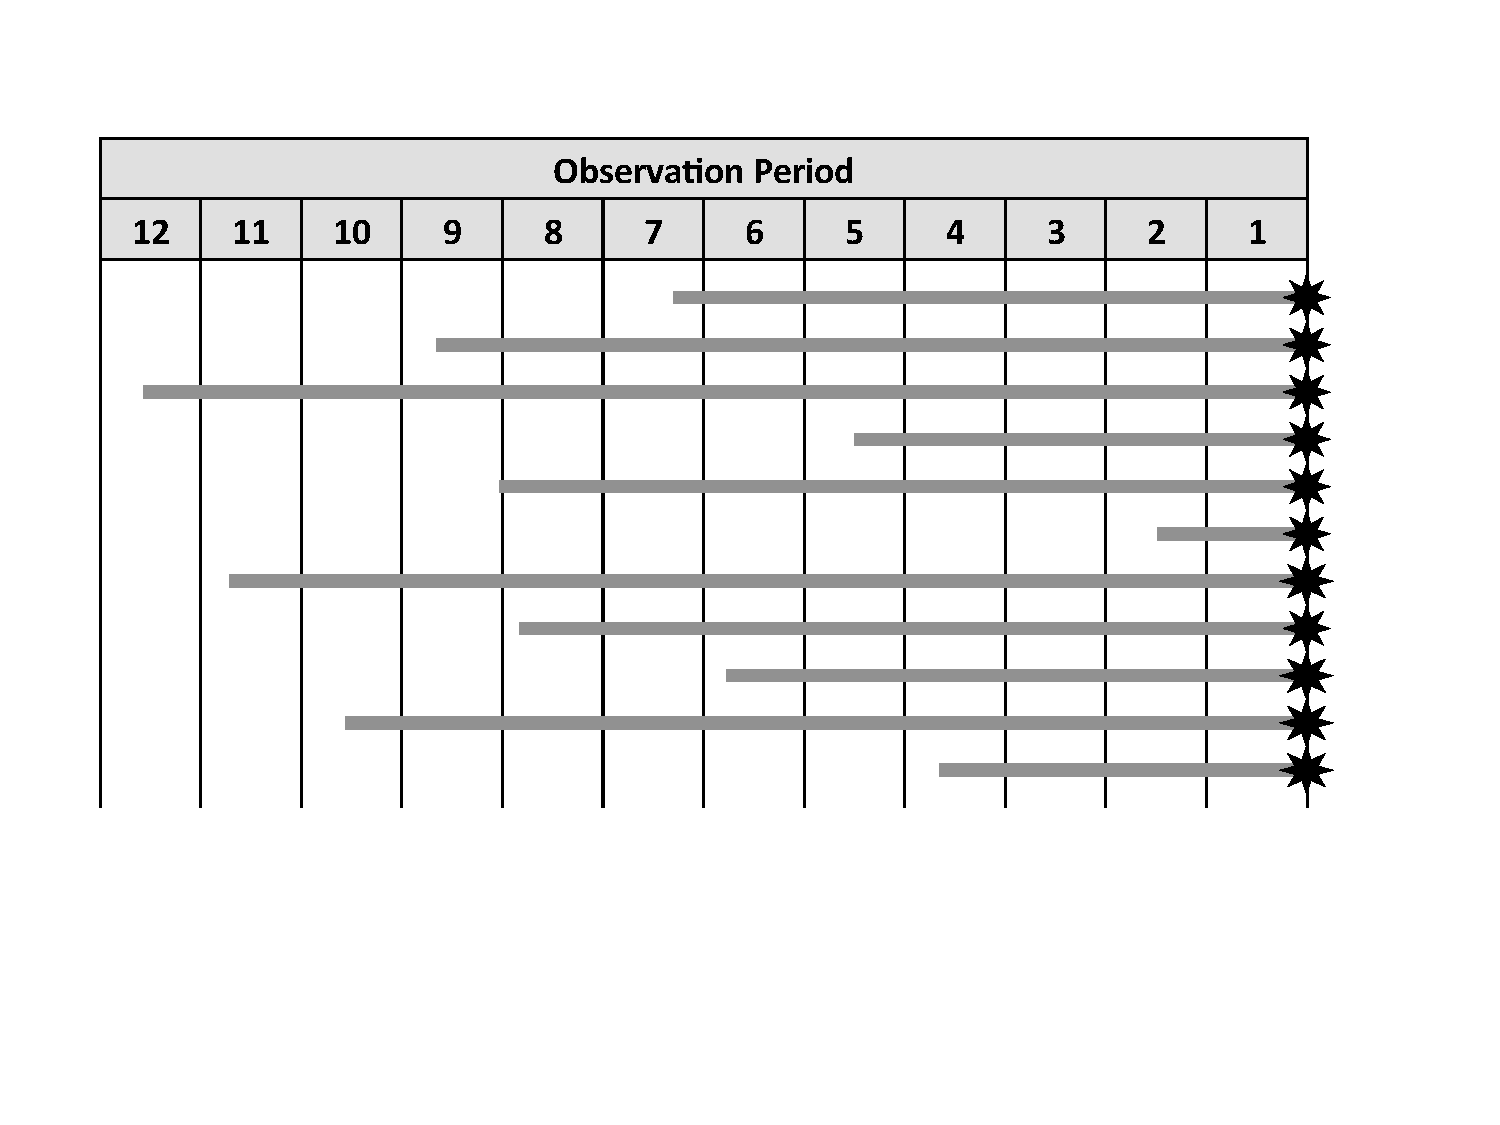
\includegraphics[width=0.49\textwidth]{./images/ModellingTimeBehaviourThenEventAligned2.pdf}}
	\end{center}
	\caption{Modeling points in time for a scenario with no real outcome period (each line represents a customer, and stars signify events).}
	\label{fig:pointInTimeDiscussionNoOutcome}
\end{figure}
\end{frame} 

 \begin{frame} 
 \begin{itemize}
\item Conversely, the target feature may have a time component and the descriptive features may not.  
\end{itemize}
\begin{figure}[htb]
	\begin{center}
			\subfigure[Actual]{\label{fig:pointInTimeDiscussion3-1}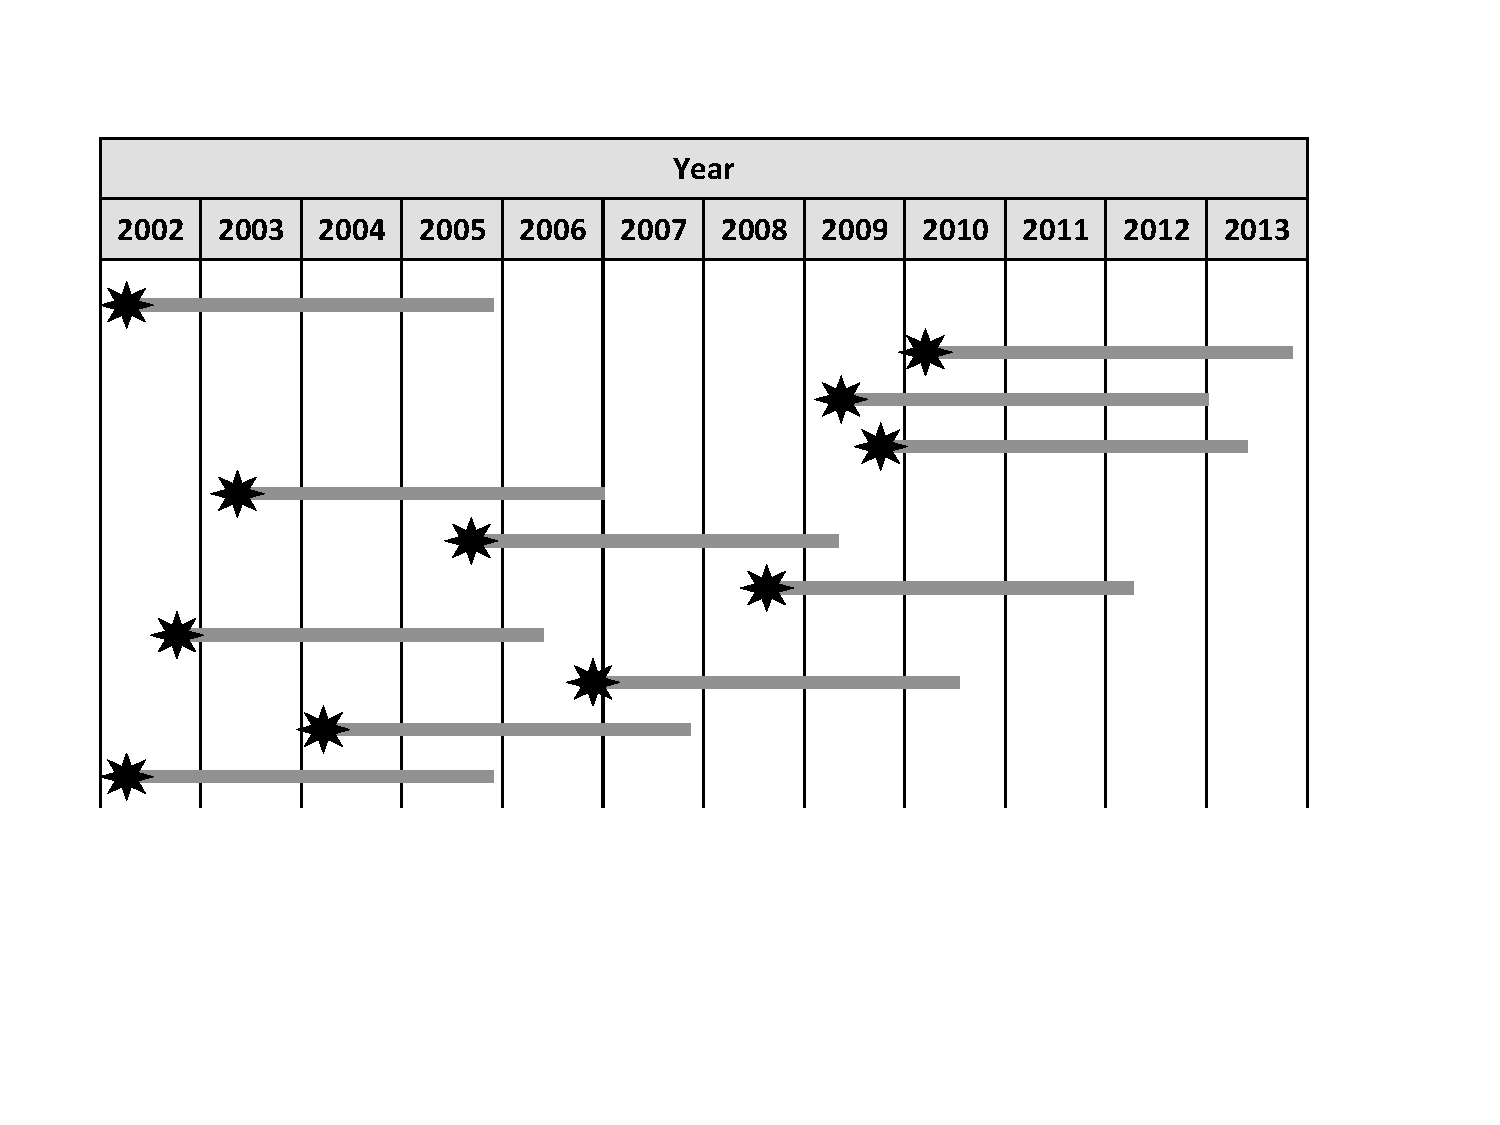
\includegraphics[width=0.49\textwidth]{./images/ModellingTimeEventThenTarget2.pdf}}
			\subfigure[Aligned]{\label{fig:pointInTimeDiscussion3-2}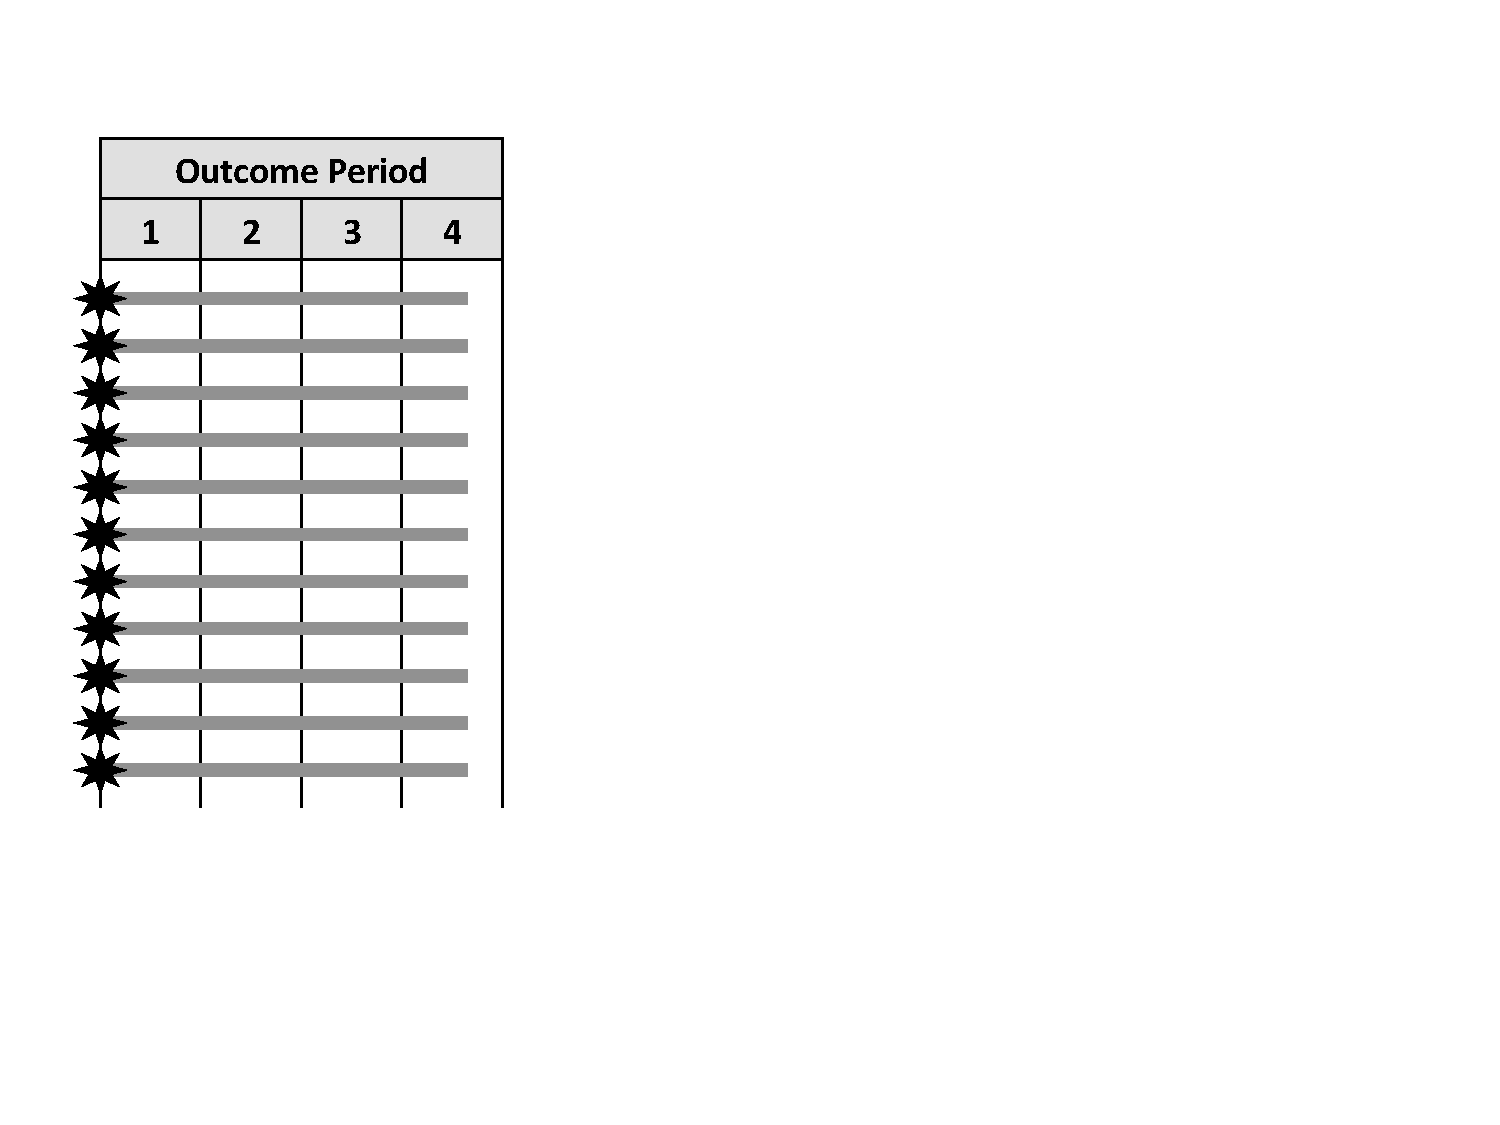
\includegraphics[width=0.18\textwidth]{./images/ModellingTimeEventThenTargetAligned2.pdf}}
	\end{center}
	\caption{Modeling points in time for a scenario with no real observation period  (each line represents a customer, and stars signify events).}
	\label{fig:pointInTimeDiscussion3}
\end{figure}
\end{frame} 


\subsection{Legal Issues}

\begin{frame}
\begin{itemize}
\item Data analytics practitioners can often be frustrated by legislation that stops them from including features that  appear to be particularly well suited to an analytics solution in an ABT. 
\item There are significant differences in legislation in different jurisdictions, but a couple of key relevant principles almost always apply.
\begin{enumerate}
\item \keyword{Anti-discrimination legislation}   
\item \keyword{Data protection legislation}
\end{enumerate}
\end{itemize}
\end{frame}

\begin{frame}
\begin{itemize}
\item Although, data protection legislation changes significantly across different jurisdictions, there are some common tenets on which there is broad agreement which affect the design of ABTs
\begin{itemize}
\item The \keyword{collection limitation principle}
\item The \keyword{purpose specification principle}
\item The \keyword{use limitation principle}
\end{itemize}
\end{itemize}
\end{frame}


\subsection{Implementing Features}

\begin{frame}
\begin{itemize}
\item Implementing a \indexkeyword{derived feature}, however, requires data from multiple sources to be combined into a set of single feature values.
\item A few key \keyword{data manipulation} operations are frequently used to calculate derived feature values: 
\begin{itemize}
\item joining data sources
\item filtering rows in a data source
\item filtering fields in a data source
\item deriving new features by combining or transforming existing features
\item aggregating data sources
\end{itemize}
\end{itemize}
\end{frame}


\subsection{Case Study: Motor Insurance Fraud}


\begin{frame}
\begin{block}{Case Study: Motor Insurance Fraud}
\begin{itemize}
\item <1-4> What are the observation period and outcome period for the motor insurance claim prediction scenario? 
\item <2-4> The observation period and outcome period are measured over different dates for each insurance claim, defined relative to the specific date of that claim.
\item <3-4> The observation period is the time prior to the claim event, over which the descriptive features capturing the claimant's behavior are calculated
\item <4> The outcome period is the time immediately after the claim event, during which it will emerge whether the claim is fraudulent or genuine.
\end{itemize}
\end{block}
\end{frame}

 \begin{frame} [plain]
 \begin{block}{Case Study: Motor Insurance Fraud}
What features could you use to capture the Claim Frequency domain concept?
\begin{figure}[htb]
	\begin{center}
			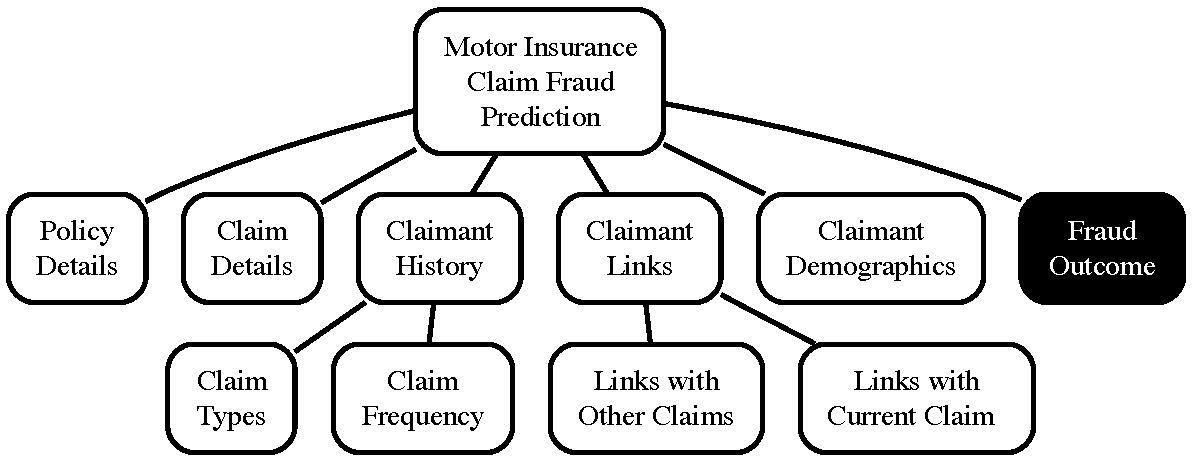
\includegraphics[width=0.9\textwidth]{./images/motorInsurance1.pdf}
	\end{center}
	\caption{Example domain concepts for a motor insurance fraud prediction analytics solution.}
	\label{fig:DataMetrics3}
\end{figure}
\end{block}
\end{frame} 

 \begin{frame} [plain]
  \begin{block}{Case Study: Motor Insurance Fraud}
  What features could you use to capture the Claim Frequency domain concept?
\begin{figure}[htb]
	\begin{center}
			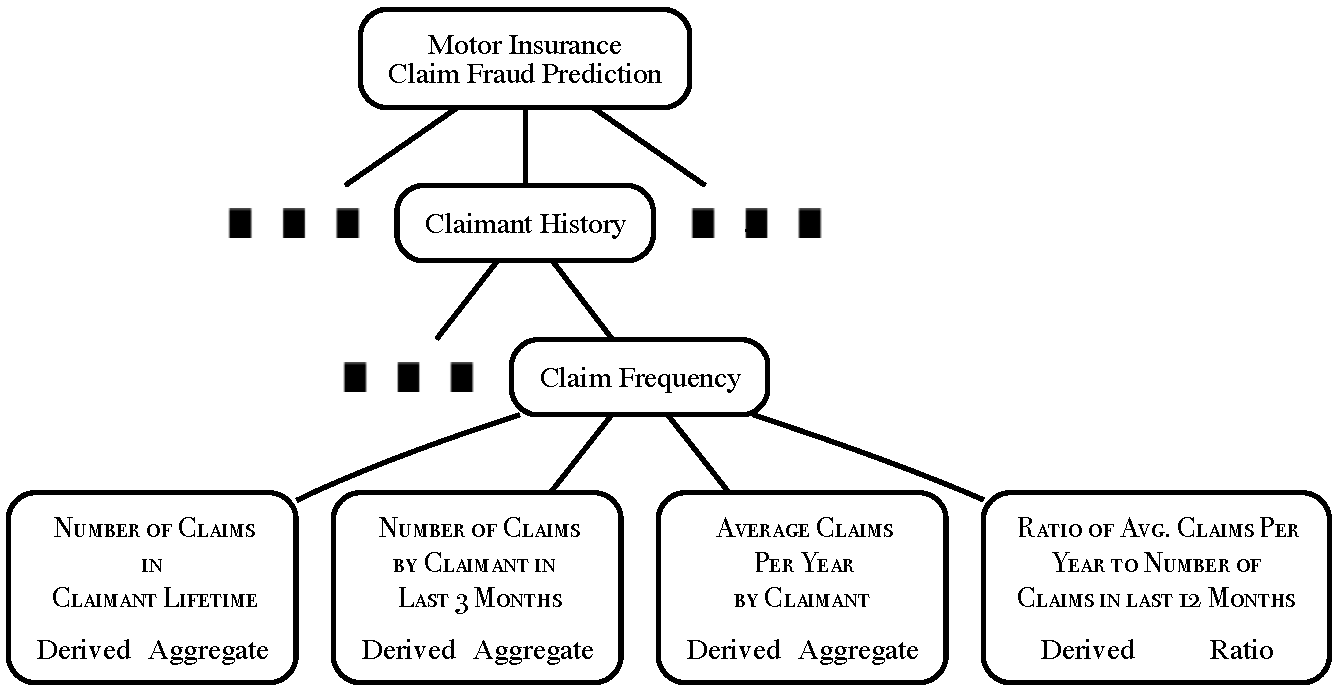
\includegraphics[width=\textwidth]{./images/motorInsurance2_SMCAPS.pdf}
	\end{center}
	\caption{A subset of the domain concepts and related features for a motor insurance fraud prediction analytics solution.}
	\label{fig:metricExample1}
\end{figure}
 \end{block}
\end{frame} 

 \begin{frame} [plain]
 \begin{block}{Case Study: Motor Insurance Fraud}
What features could you use to capture the Claim Types domain concept?
\begin{figure}[htb]
	\begin{center}
			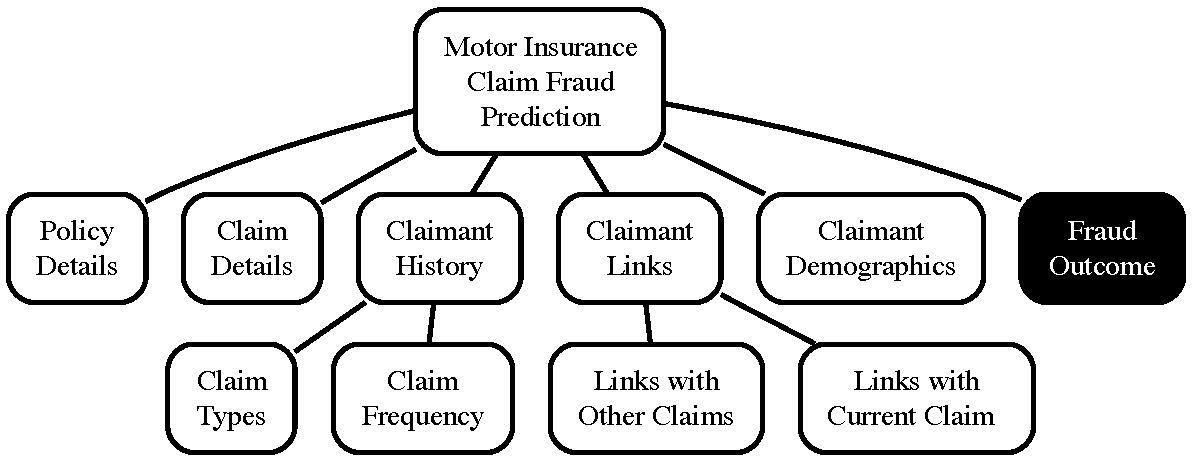
\includegraphics[width=0.9\textwidth]{./images/motorInsurance1.pdf}
	\end{center}
	\caption{Example domain concepts for a motor insurance fraud prediction analytics solution.}
	\label{fig:DataMetrics3}
\end{figure}
\end{block}
\end{frame} 

 \begin{frame} [plain]
 \begin{block}{Case Study: Motor Insurance Fraud}
What features could you use to capture the Claim Types domain concept?
\begin{figure}[htb]
	\begin{center}
			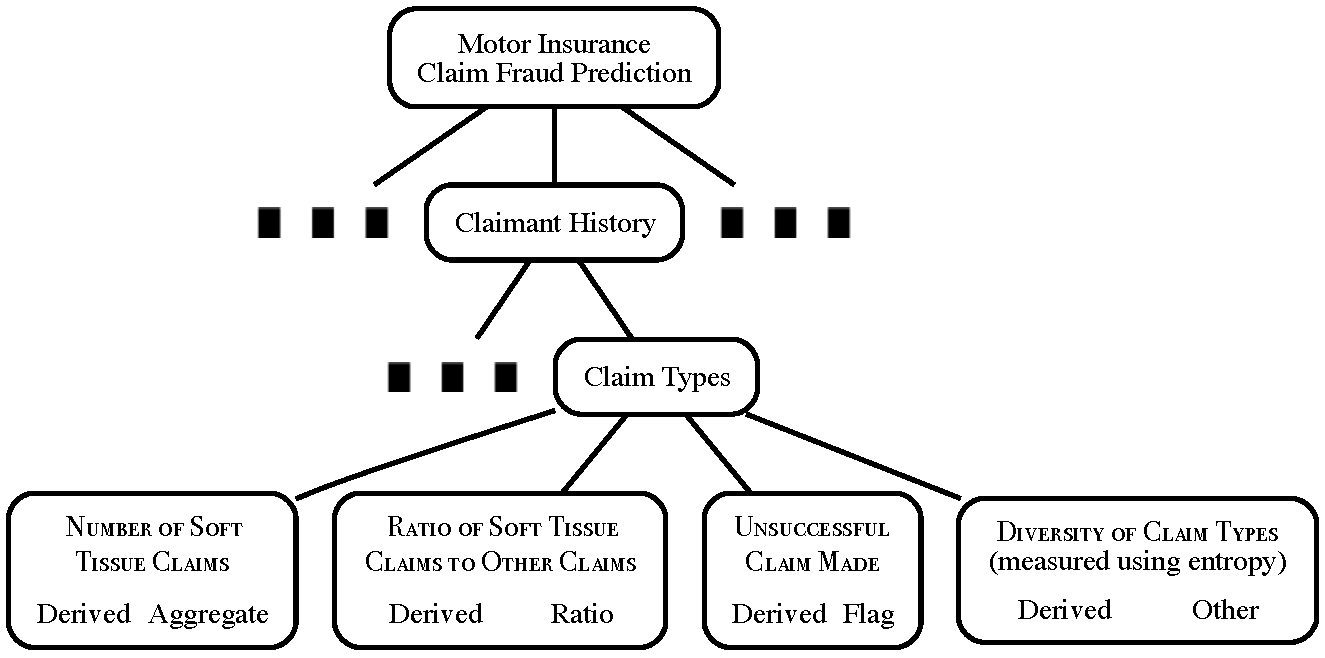
\includegraphics[width=\textwidth]{./images/motorInsurance3_SMCAPS.pdf}
	\end{center}
	\caption{A subset of the domain concepts and related features for a motor insurance fraud prediction analytics solution.}
	\label{fig:metricExample2}
\end{figure}
\end{block}
\end{frame} 


 \begin{frame} [plain]
 \begin{block}{Case Study: Motor Insurance Fraud}
What features could you use to capture the Claim Details domain concept?
\begin{figure}[htb]
	\begin{center}
			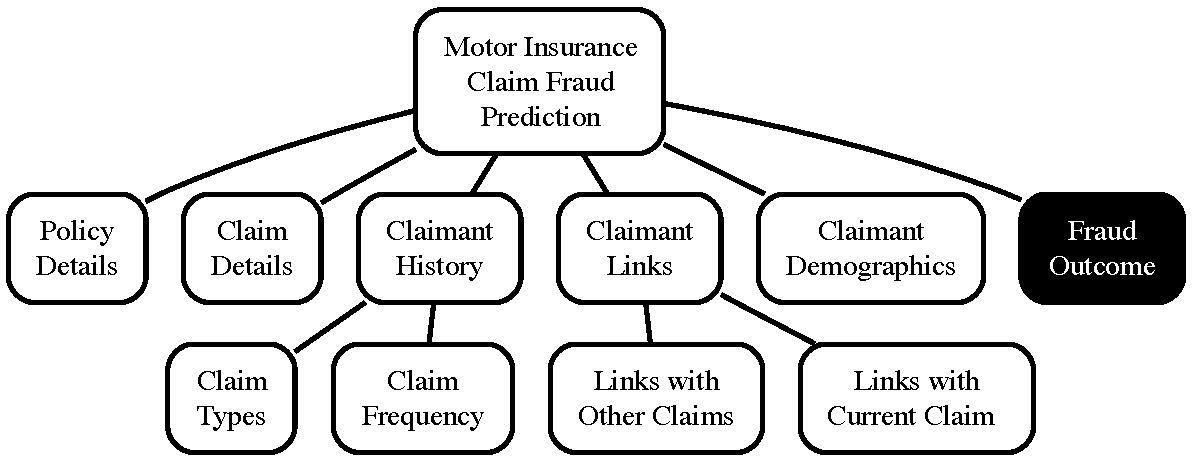
\includegraphics[width=0.9\textwidth]{./images/motorInsurance1.pdf}
	\end{center}
	\caption{Example domain concepts for a motor insurance fraud prediction analytics solution.}
	\label{fig:DataMetrics3}
\end{figure}
\end{block}
\end{frame} 

 \begin{frame} [plain]
 \begin{block}{Case Study: Motor Insurance Fraud}
What features could you use to capture the Claim Details domain concept?
\begin{figure}[htb]
	\begin{center}
			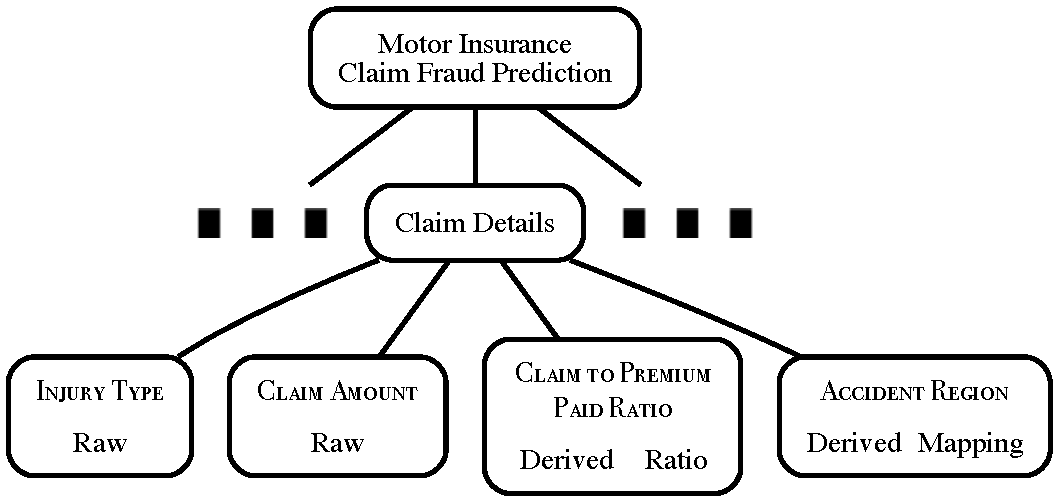
\includegraphics[width=0.8\textwidth]{./images/motorInsurance4_SMCAPS.pdf}
	\end{center}
	\caption{A subset of the domain concepts and related features for a motor insurance fraud prediction analytics solution.}
	\label{fig:metricExample3}
\end{figure}
\end{block}
\end{frame} 


\begin{frame}
 \begin{block}{Case Study: Motor Insurance Fraud}
\begin{itemize}
\item The following table illustrates the structure of the final ABT that was designed for the motor insurance claims fraud detection solution. 
\item The table contains more descriptive features than the ones we have discussed
\item The table also shows the first four instances. 
\item If we examine the table closely, we see a number of strange values (for example, $-9\,999$) and a number of missing values---we will return to these in Chapter 3.
\end{itemize}
\end{block}
\end{frame}


 \begin{frame} [plain]
\begin{table}[!tb]
\caption{The ABT for the motor insurance claims fraud detection solution.}
\label{table:fraudDetectionABT}
\begin{tiny}
\begin{tabular}{ c c r c c c c r}
\hline
	&		&		&		&		&		&		&		\\
	&		&		&	\featN{Marital}	&	\featN{Num.}	&	\featN{Injury}	&	\featN{Hospital}	&	\featN{Claim}	\\
\featN{ID}	&	\featN{Type}	&	\featN{Inc}.	&	\featN{Status}	&	\featN{Clmnts.}	&	\featN{Type}	&	\featN{Stay}	&	\featN{Amt.}	\\
	\hline
1	&	CI	&	0	&		&	2	&	Soft Tissue	&	No	&	1\,625	\\
2	&	CI	&	0	&		&	2	&	Back	&	Yes	&	15\,028	\\
3	&	CI	&	54\,613	&	Married	&	1	&	Broken Limb	&	No	&	-9\,999	\\
4	&	CI	&	0	&		&	3	&	Serious	&	Yes	&	270\,200	\\	
\multicolumn{5}{c}{\textbf{\vdots}} & \multicolumn{3}{c}{\textbf{\vdots}}\\
\hline
\end{tabular}
\vspace{0.2in}\\
\begin{tabular}{ c r c c c c c c}
\hline
	&		&		&	\featN{Num.}	&	\featN{Avg.}	&	\featN{Avg.}	&	\featN{Num.}	&	\featN{\%}	\\
	&	\featN{Total}	&	\featN{Num.}	&	\featN{Claims} &	\featN{Claims}	&	\featN{Claims}	&	\featN{Soft}	&	\featN{Soft}	\\
\featN{ID}	&	\featN{Claimed}	&	\featN{Claims}	&	\featN{3 Months} &	\featN{Per Year}	&	\featN{Ratio}	&	\featN{Tissue}	&	\featN{Tissue}	\\
	\hline
1	&	3\,250	&	2	&	0	&	1	&	1	&	2	&	1	\\
2	&	60\,112	&	1	&	0	&	1	&	1	&	0	&	0	\\
3	&	0	&	0	&	0	&	0	&	0	&	0	&	0	\\
4	&	0	&	0	&	0	&	0	&	0	&	0	&	0	\\
\multicolumn{4}{c}{\textbf{\vdots}} & \multicolumn{4}{c}{\textbf{\vdots}}\\
	\hline
\end{tabular}
\vspace{0.2in}\\
\begin{tabular}{ c c r c c c c }
\hline
	&		&	\featN{Claim} &		&	\featN{Claim}	&		&		\\
	&	\featN{Unsucc.}	&	\featN{Amt.} &	\featN{Claim}	&	\featN{to}	&		&	\featN{Fraud}	\\
\featN{ID}	&	\featN{Claims}	&	\featN{Rec.}	&	\featN{Div.}	&	\featN{Prem.}	&	\featN{Region}	&	\featN{Flag}	\\
	\hline
1	&	2	&	0	&	0	&	32.5	&	MN	&	1	\\
2	&	0	&	15\,028	&	0	&	57.14	&	DL	&	0	\\
3	&	0	&	572	&	0	&	-89.27	&	WAT	&	0	\\
4	&	0	&	270\,200	&	0	&	30.186	&	DL	&	0	
	\\\multicolumn{4}{c}{\textbf{\vdots}} & \multicolumn{3}{c}{\textbf{\vdots}}\\
\hline
\end{tabular}
\end{tiny}
\end{table}
\end{frame} 


\SectionSlide{Summary}

\begin{frame}
\begin{itemize}
\item Predictive data analytics models built using machine learning techniques are tools that we can use to help make better decisions within an organization, not an end in themselves. 
\item It is important to fully understand the business problem that a model is being constructed to address---this is the goal behind \textit{converting business problems into analytics solutions}
\end{itemize}
\end{frame}


\begin{frame}
\begin{itemize}
\item Predictive data analytics models are reliant on the data that is used to build them---the \keyword{analytics base table} (\keyword{ABT}). 
\item The first step in designing an ABT is to decide on the \keyword{prediction subject}.
\item An effective way in which to design ABTs is to start by defining a set of \keyword{domain concepts} in collaboration with the business, and then designing \keyword{features} that express these concepts in order to form the actual ABT. 
\end{itemize}
\end{frame}


\begin{frame}
\begin{itemize}
\item Features (both descriptive and target) are concrete numeric or symbolic representations of domain concepts. 
\item It is useful to distinguish between \keyword{raw features} that come directly from existing data sources and \keyword{derived features} that are constructed by manipulating values from existing data sources. 
\item Common manipulations used in this process include aggregates, flags, ratios, and mappings, although any manipulation is valid. 
\end{itemize}
\end{frame}

\begin{frame}
\begin{itemize}
\item The techniques described here cover the \keyword{Business Understanding}, \keyword{Data Understanding}, and (partially) \keyword{Data Preparation} phases of the \keyword{CRISP-DM} process. 
\begin{figure}[!htb]
	\begin{center}
			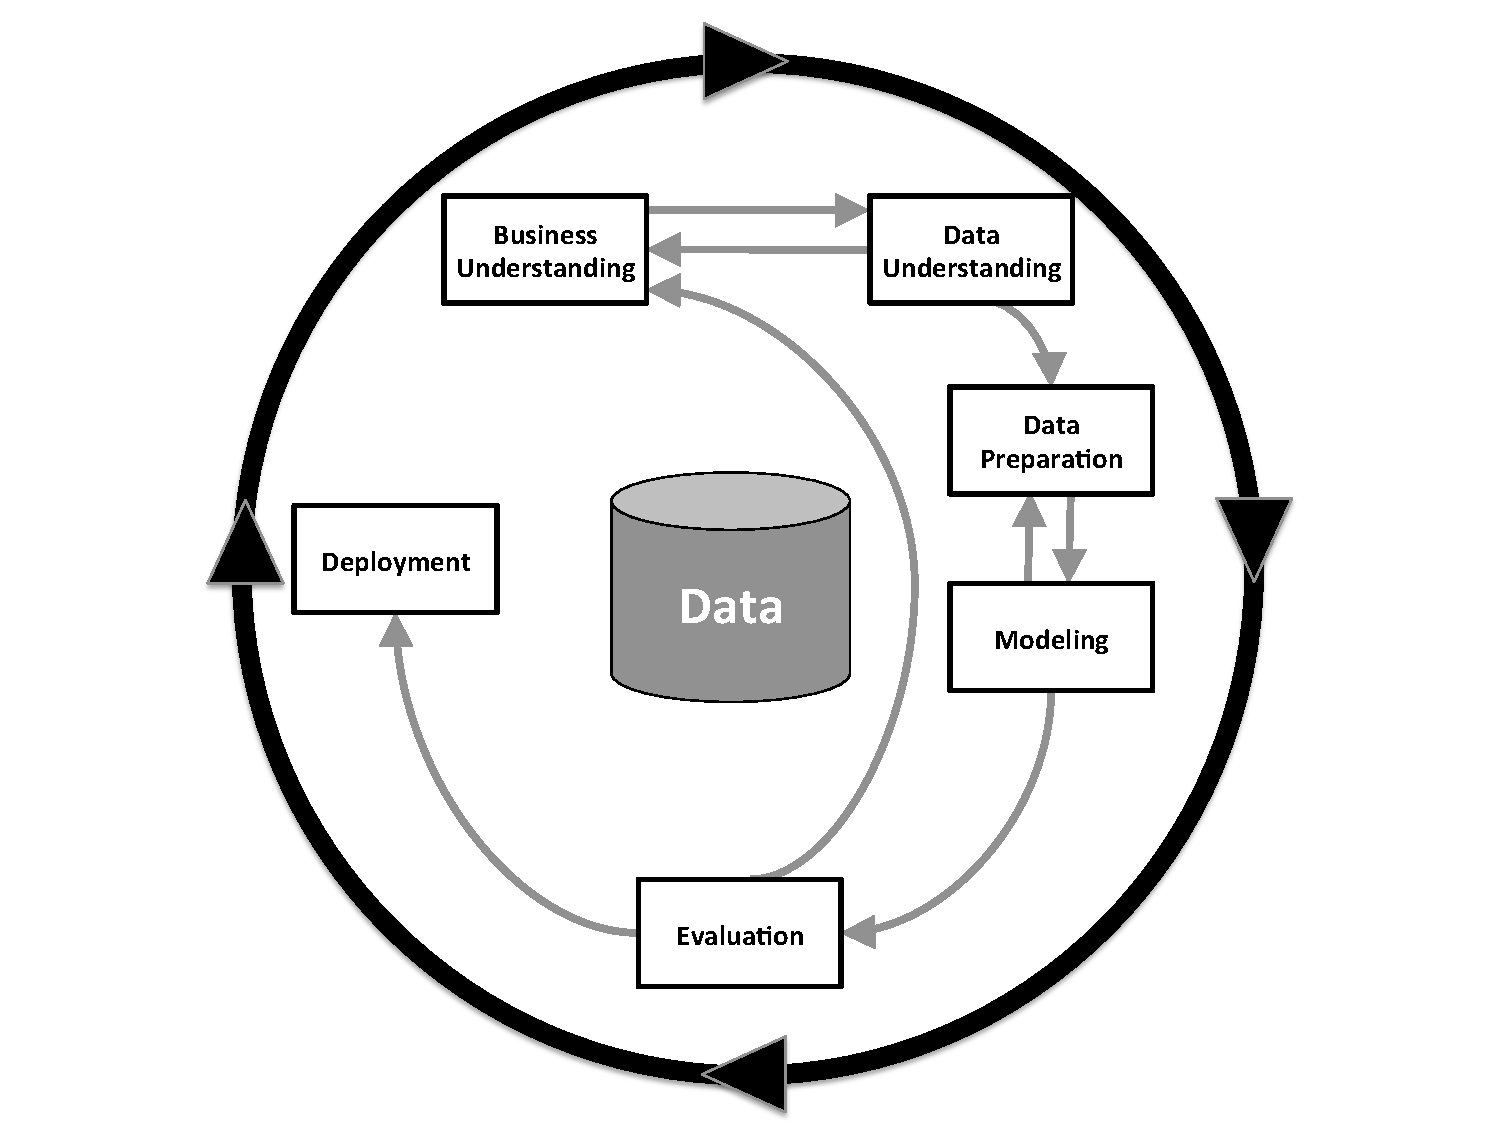
\includegraphics[width=0.5\textwidth]{./images/CrispDM_BW_mod.pdf}
	\end{center}
	\caption{A diagram of the CRISP-DM process.}
	\label{fig:crispDM}
\end{figure}

\end{itemize}
\end{frame} 

 \begin{frame} [plain]
\begin{figure}[htb]
       \begin{centering}
       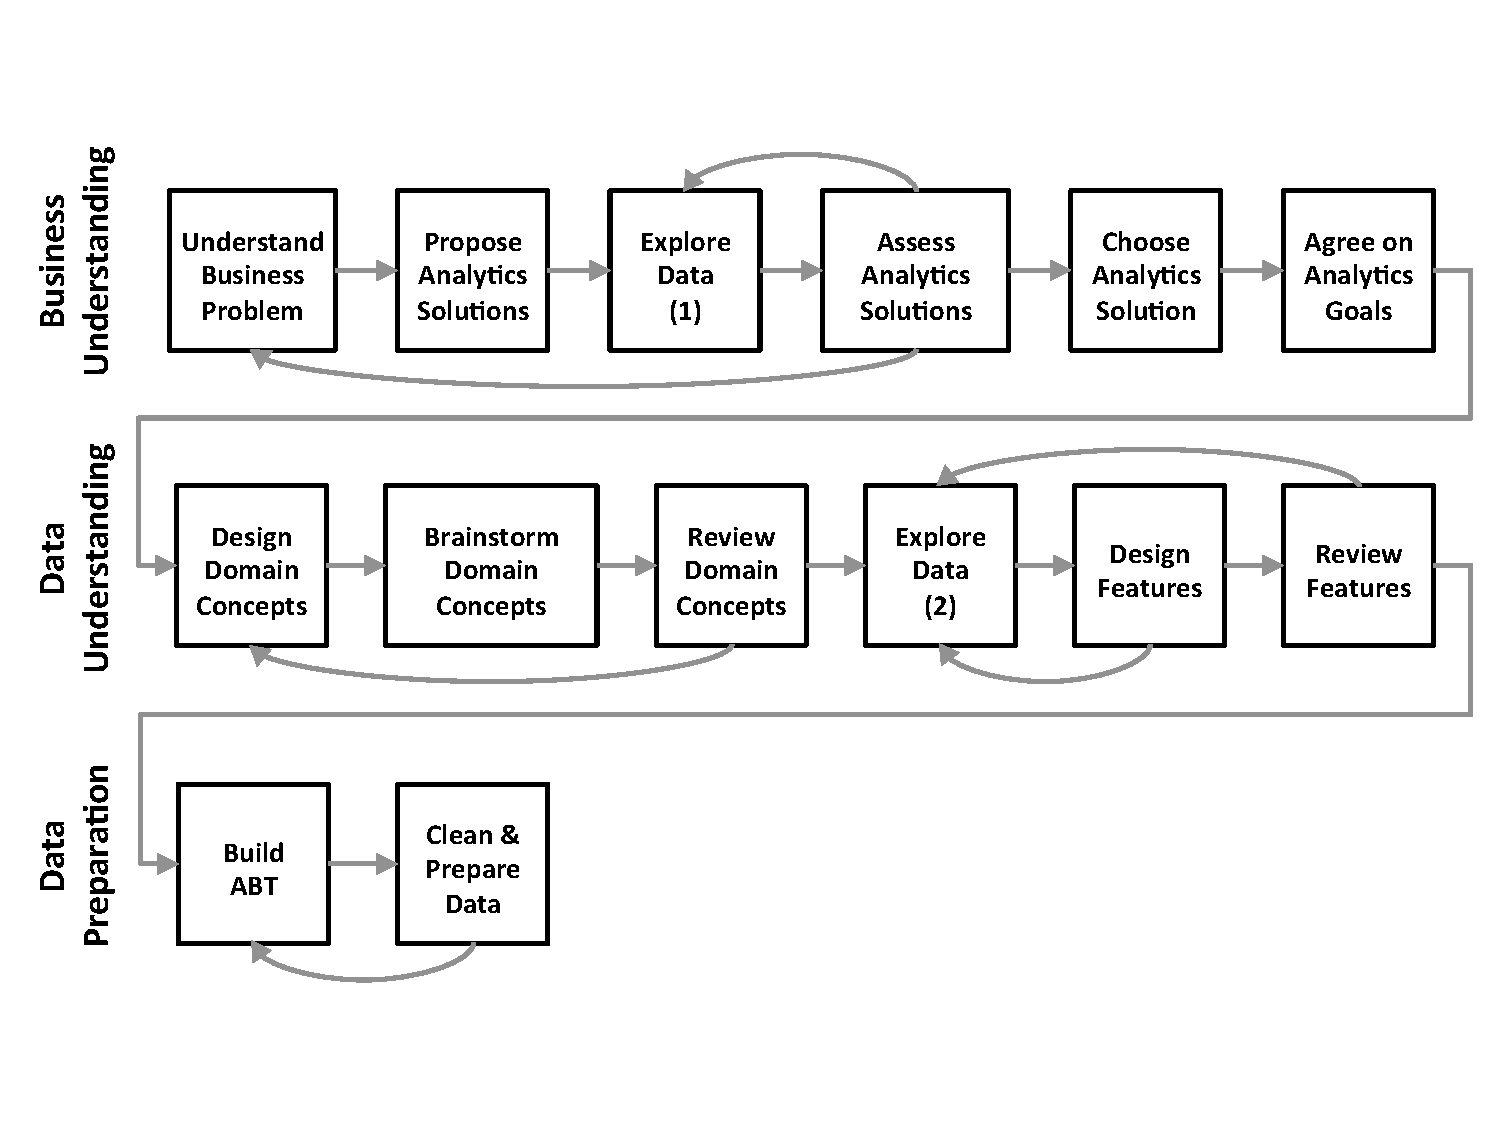
\includegraphics[width=0.99\textwidth]{images/DataInsightsDecisionsProcessSummary3.pdf}
       \caption{A summary of the tasks in the Business Understanding, Data Understanding, and Data Preparation phases of the \indexkeyword{CRISP-DM} process.}
       \label{fig:processSummaryDiagram}
       \end{centering}
\end{figure}
\end{frame} 

\begin{frame}
	\tableofcontents
\end{frame}

\end{document}
